
\documentclass[mathserif, aspectratio=169]{beamer}

\usepackage{psfrag,graphicx}
\usepackage{amsmath}
\usepackage[absolute,overlay]{textpos}

\usepackage{braket}
\graphicspath{{figs/}}

\usetheme{Boadilla}
\makeatother
\setbeamertemplate{footline}[frame number]

\usepackage{graphicx}
\usepackage{caption}
\usepackage{subcaption}
\captionsetup{compatibility=false}
\usepackage{amsmath} 
\usepackage{amssymb} 
\usepackage{amsthm}  
\usepackage{bm}
\usepackage{lipsum}
\usepackage[linesnumbered, ruled]{algorithm2e}
\usepackage{color}
\newtheorem{assumption}{Assumptions}
\newtheorem{prop}{Proposition}
\newtheorem{defn}{Definition}
\newtheorem{thm}{Theorem}
\newtheorem{lem}{Lemma}
\newtheorem{cor}{Corollary}
\newtheorem{sol}{Decentralized Solution}
\newtheorem{thresh}{$\epsilon$-thresholding}
\definecolor{light-gray}{gray}{0.8}
\usepackage{textcomp}

\newcommand{\backupbegin}{
   \newcounter{finalframe}
   \setcounter{finalframe}{\value{framenumber}}
}
\newcommand{\backupend}{
   \setcounter{framenumber}{\value{finalframe}}
}
\newcommand{\norm}[1]{\left\lVert #1 \right\rVert}

\makeatletter
\setbeamertemplate{navigation symbols}{}

\title[Lecture 25] 
{Data, Environment and Society: \\{Lecture 25: Neural Networks}}



\author[ER131: Data, Environment and Society] 
{Instructor: Duncan Callaway\\
GSI: Salma Elmallah} 

%\logo{
%\includegraphics[width=1.5cm,height=1.5cm,keepaspectratio]{uvic_logo_h.jpg}
%}
\vspace{-20mm}
\institute[UC Berkeley] % (optional, but mostly needed)
 {\small{ \bf November 26, 2019}}

\date[November 26, 2019]

\begin{document}

\frame{
	\titlepage
}


\begin{frame}{Announcements}
	\begin{itemize}
		\item HW10 due today
		\item Next today and tuesday: neural nets
		\begin{itemize}
			\item Feel free to use on projects -- but no HW here.
		\end{itemize}
		\item Course evaluations available online; I will make time next Tuesday
		\item Thursday: Career panel
		\begin{itemize}
			\item JP Dolphin, manager of Strategic Data Science at PG\&E
			\item Tanner Burke, senior data engineer, Streetlight Data
			\item Jason Harville, assistant executive director of the Energy Data and Analytics Office, California Energy Commission
		\end{itemize}
	\end{itemize}
\end{frame}


\begin{frame}{Today's outline}
	\begin{enumerate}
		\item Neural networks (NN) 
		\begin{itemize}
			\item  Brief introduction
			\item Experiment with tensorflow playground -- try fitting different classification problems
			\item Objective: Understand the role of key parameters, what the hyperparameters are, and the model fitting process
		\end{itemize}
		\item Exam handout and discussion
	\end{enumerate}
\end{frame}


\begin{frame}
	\frametitle{Neural networks: Origins}
	\begin{columns}[c]
		\column{0.5\textwidth}
			\begin{itemize}
				\item The name is due to analogy with brains
				\item First developed in 1943
				\item Inspired the development of the perceptron (see HW10) in the `50s
				\begin{itemize}
					\item Here the purpose was just to remove noise on phone lines
					\item Not to reproduce thought...
				\end{itemize}
				\item Little research activity $\sim$1960-1990's due to computing limitations
				\begin{itemize}
					\item Major exception: Werbos developed back-propogation in 1974.  First effort to get NN to ``learn'' parameters
				\end{itemize}
				\item Computing advances made ``deep'' NN possible in the last 20 years
			\end{itemize}
		\column{0.5\textwidth}
			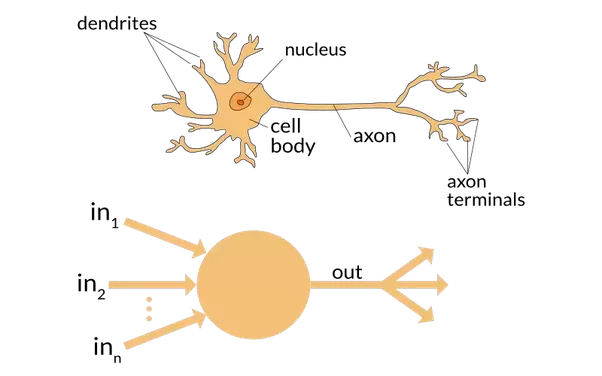
\includegraphics[width=\textwidth]{nn_v_ann}
	\end{columns}
\end{frame}


\begin{frame}{Mathematics for a single ``neuron''}   
    \begin{columns}
    	\column{0.5\textwidth}
    		In words, each neuron...
    		\begin{itemize}
    			\item Takes a vector of values as inputs
    			\item Creates a scalar from a linear combination of the vector entries
    			\item Passes the resulting scalar through an ``activation function''
    			\item Outputs a single value from that activation function
    		\end{itemize}

    		Terminology analogies:
    		\begin{itemize}
    			\item Electrical signal from other cells $\rightleftarrows$ input
    			\item Neuron $\rightleftarrows$ Activation function
    			\item Electrical signal to other cells $\rightleftarrows$ output
    		\end{itemize}
    	\column{0.5\textwidth}
    	\pause
    	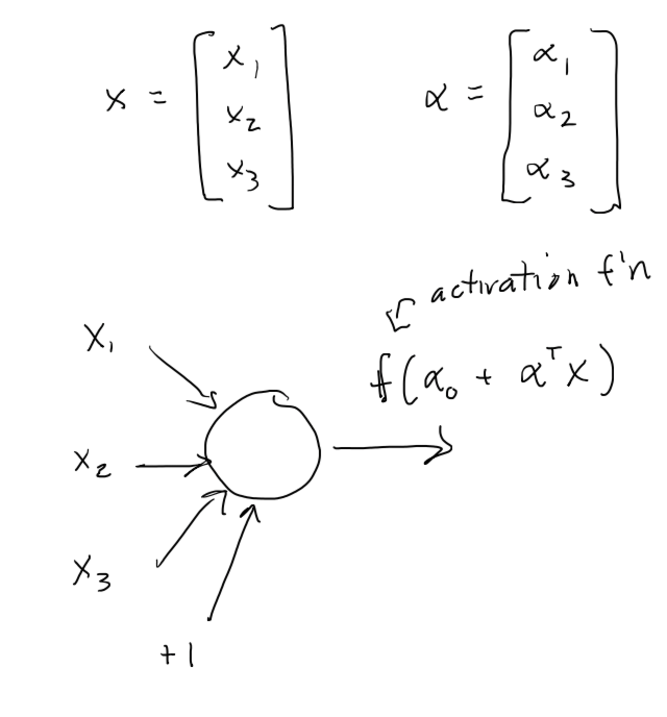
\includegraphics[width=0.85\textwidth]{neuron_math.pdf}
	    	
    \end{columns}
\end{frame}


\begin{frame}[t]\frametitle{What's $f$, the activation function?}
    \begin{columns}
	    \column{0.3\textwidth}
	    \begin{enumerate}
	    	\item sigmoid
	    	\vspace{15mm}
	    	\item $\tanh$
	    	\vspace{15mm}
	       	\item rectified linear (ReLU)
	    \end{enumerate}
	    \column{0.7\textwidth}
	    \pause
        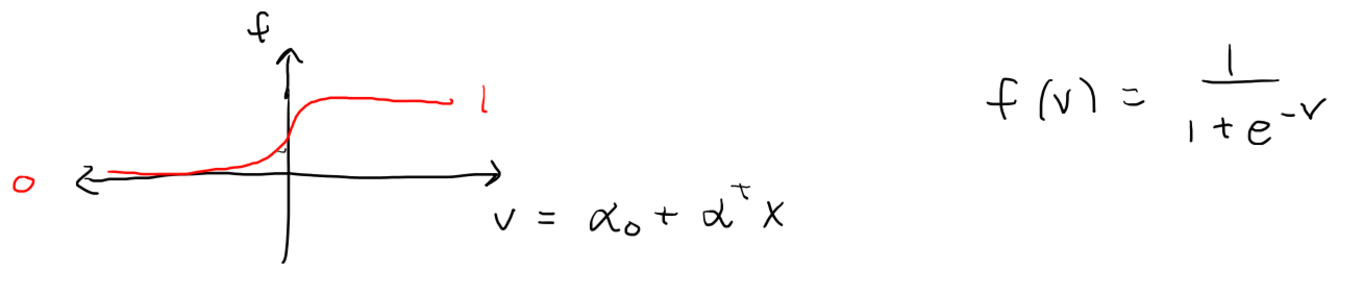
\includegraphics[width = 1\textwidth]{sigmoid.pdf}

    	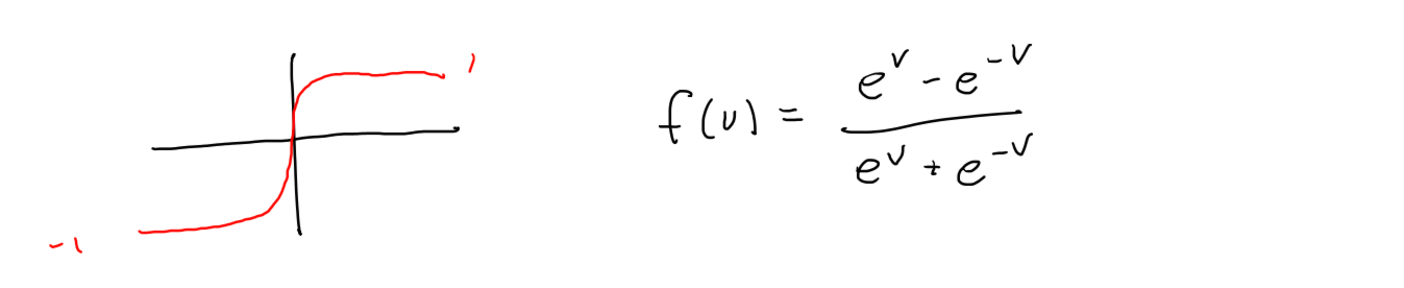
\includegraphics[width = 1\textwidth]{tanh.pdf}

		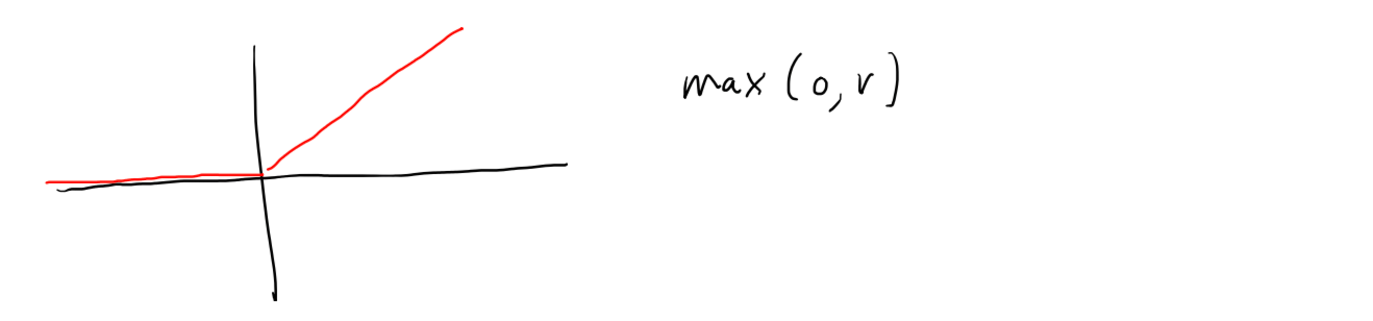
\includegraphics[width = 1\textwidth]{rectilinear.pdf}

    \end{columns}
\end{frame}



\begin{frame}[t]\frametitle{How the sigmoid function works}
    
    \pause
    \begin{columns}

    \column{0.7\textwidth}
	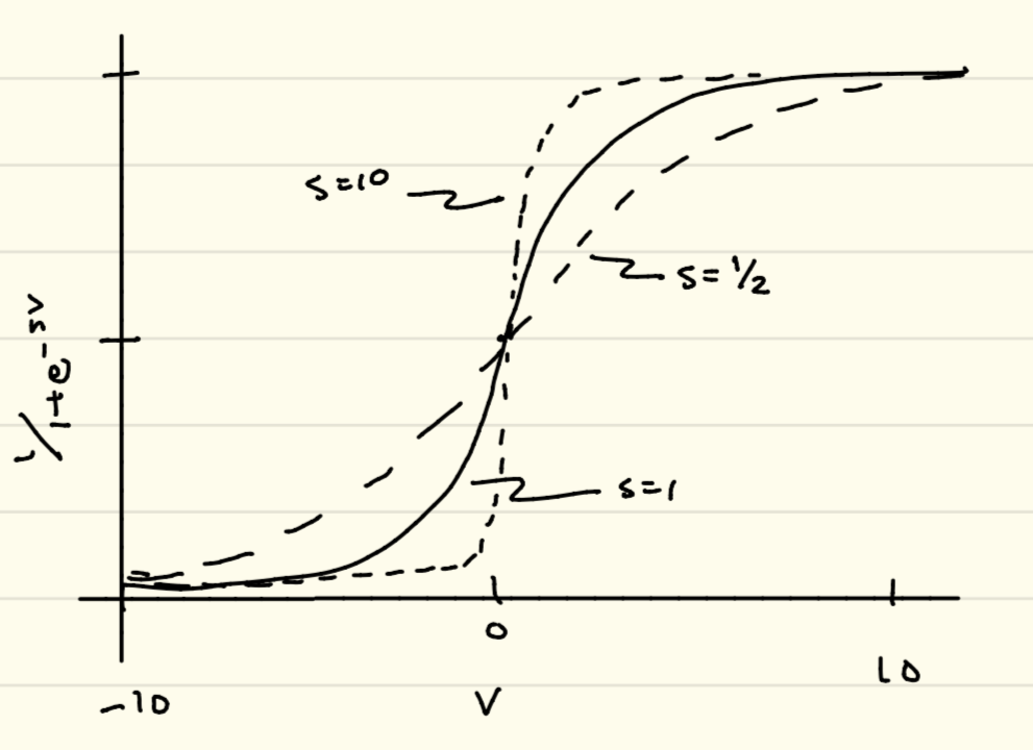
\includegraphics[height = 0.9\textheight]{sigmoid_examples.pdf}
	\column{0.3\textwidth}
	Remember: $v = \alpha_0 + \alpha^T \mathbf{x}$
	\end{columns}
\end{frame}

\begin{frame}[t]\frametitle{Neural network: just gang the neurons together}
    
    \pause

	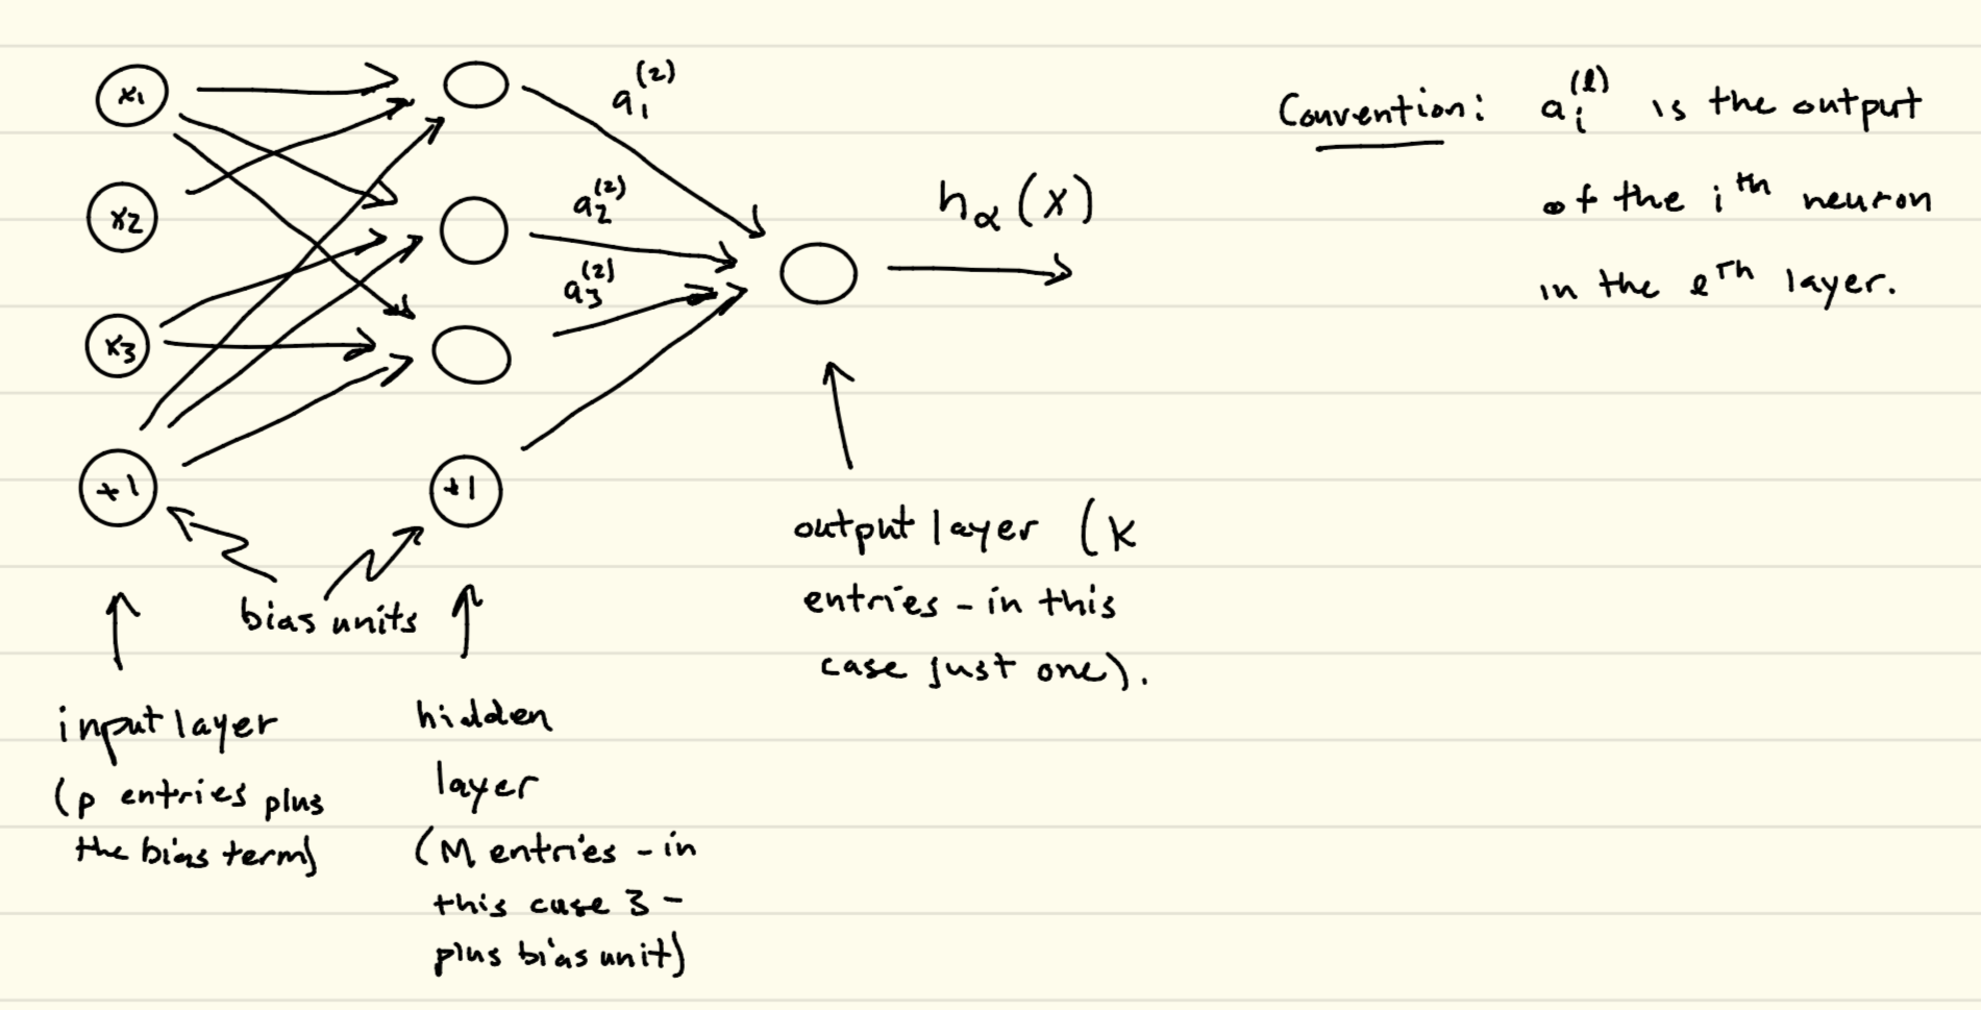
\includegraphics[height = 0.9\textheight]{NN.pdf}
\end{frame}


\begin{frame}[t]\frametitle{Mathematical merging of neurons}
    Convention:
    \begin{itemize}
    	\item $\alpha_{ij}^{(l)} \rightarrow$ weight from node $j$ in layer\\ $l$ to node $i$ in $l+1$ layer.
    	\item $a_{i}^{(l)} \rightarrow$ output of node $i$ in layer $l$.
    %	\item $z_i^{(l)} \rightarrow$ input into node $i$ in layer $l$.
    \end{itemize}

    \begin{columns}
    	\column{0.5\textwidth}
    	    \begin{align*}
		     	a_1^{(2)} &= \uncover<2->{f(\alpha_{10}^{(1)} + \alpha_{11}^{(1)}x_1^{(1)}+\alpha_{12}^{(1)}x_2^{(1)}+\alpha_{13}^{(1)}x_3^{(1)})} \\
		     	a_1^{(3)} &= \uncover<2->{f(\alpha_{10}^{(2)} + \sum_{j=1}^M\alpha_{1j}^{(2)}a_j^{(2)})} \\
		    \end{align*}
	    \column{0.5\textwidth}
    \end{columns}
    Note that I used $x$ in the first equation because I'm calling the features (inputs to the model) the first ``layer'' of the network
	
    \textbf{Question}: What are the parameters of a neural network model?

    \uncover<2->{    Just the $\alpha$ values.  $a$ values are outputs from internal nodes or neurons.  We call these ``hidden states'' because they depend on the input values $x$.  }
\end{frame}

\begin{frame}[t]\frametitle{Thinking about the features and target}
    Let's watch this video.  It uses graphics in a nice way to explain what NNs are doing. 
    \vspace{10mm}

    \url{https://www.youtube.com/watch?v=aircAruvnKk}

    \vspace{10mm}

    Start the video at 2:05.  We'll stop watching around 5:30.
\end{frame}

\begin{frame}{Compact notation motivates a name...}
	\pause
	\begin{align*}
		a^{(2)}_i &= f(\alpha_{i0}^{(1)} + \alpha_{i1}^{(1)}x_1^{(1)}+\alpha_{i2}^{(1)}x_2^{(1)}+\alpha_{i3}^{(1)}x_3^{(1)})\\
		a^{(3)}_i & = f(\alpha_{i0}^{(2)} + \sum_{j=1}^{M_2} \alpha_{ij}^{(2)}a_j^{(2)}) \quad (M_j \text{ is the number of neurons in layer $j$})\\
		a^{(4)}_i & = f(\alpha_{i0}^{(3)} + \sum_{j=1}^{M_3} \alpha_{ij}^{(3)}a_j^{(3)})\\
		&\vdots\\
		h_\alpha(x) &= f(a^{(\ell)}, \alpha^{(\ell)}) \quad \text{Final output of NN. }\ell \text{ is the number of layers}
	\end{align*}

	\begin{itemize}
		\item The $_\alpha$ subscript means $h$ is a function of ALL the $\alpha$ values of the network
		\item We dropped subscripts on $a$, meaning $a$ is a vector of inputs to the final layer
	\end{itemize}
	Because each layer informs the next, we call this a \textbf{feedforward} neural network.
\end{frame}

\begin{frame}[t]\frametitle{Fitting the model - regression}
	Training data: $\{(x_1,y_1), (x_2,y_2), \hdots, (x_n,y_n)\}$

	\vspace{5mm}

	$x \in \mathbb{R}^p$ ($p$ features), single output, $y$

	\vspace{5mm}
	Objective function: 
	\pause

	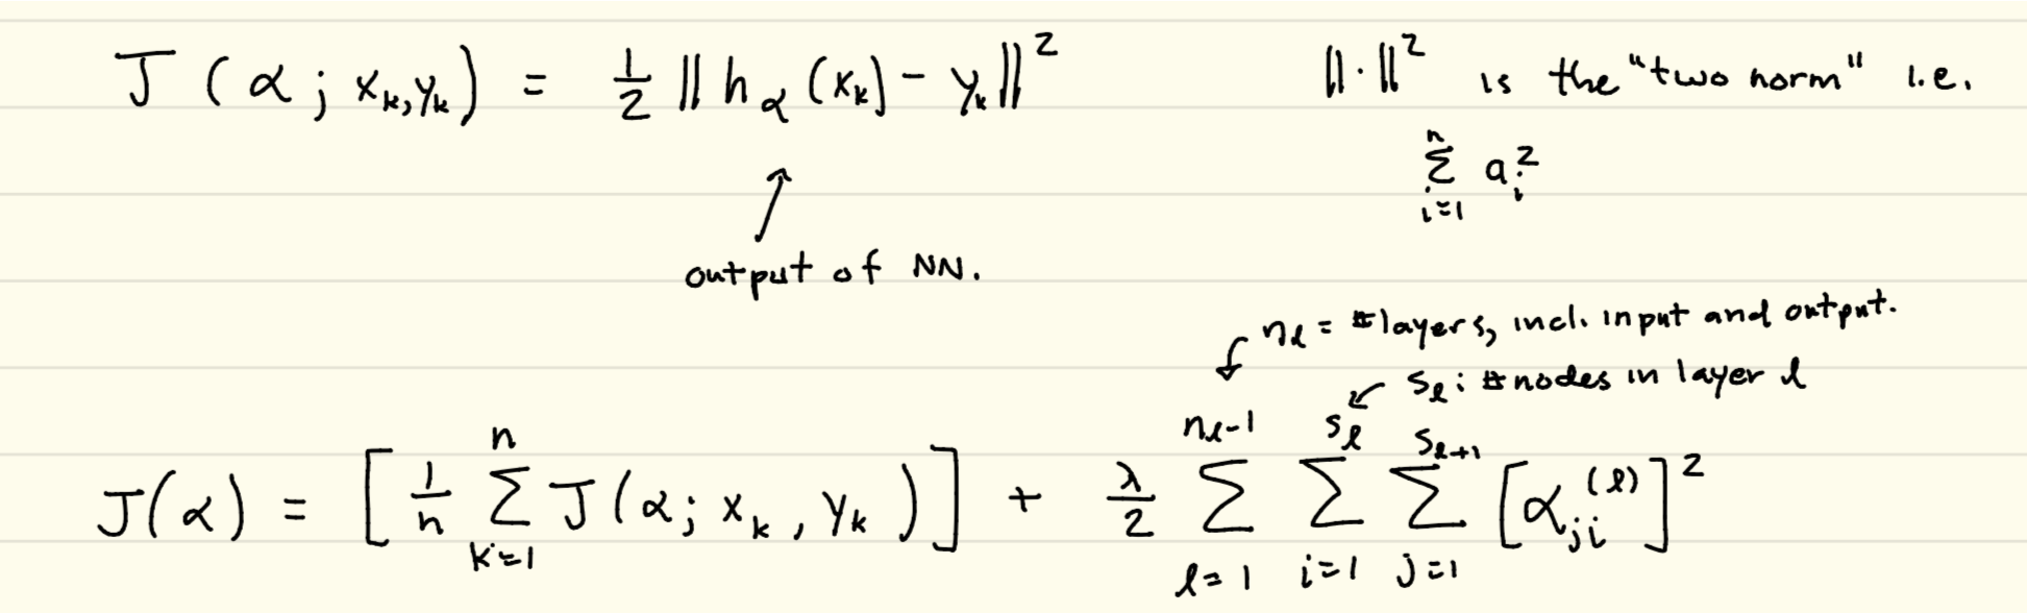
\includegraphics[width = 0.9\textwidth]{NN_J}

\end{frame}

\begin{frame}[t]\frametitle{Quick notes on objective function and finding parameters}
    
	\begin{itemize}
	 	\item Form is amenable to classification, just one-hot encode the output and use classification error rate as your objective
	 	\item For regression, be sure to scale the \textit{output} variables to lie in the range of the activation function. 
	 	\begin{itemize}
	 		\item For sigmoid, scale to: \pause $[0,1]$
	 		\item Tanh: \pause $[-1,1]$
	 		\pause
	 		\item (I \textit{believe} ReLU requires shifting output to be non-negative; textbook does not address.)
	 	\end{itemize}
	 	\item Solving the objective function involves a form of gradient search
	 	\begin{itemize}
	 	 	\item The partial derivatives are found via a technique called backpropogation
	 	 \end{itemize} 
	\end{itemize} 

\end{frame}

\begin{frame}[t]\frametitle{Tensorflow playground}
    On \href{http://playground.tensorflow.org}{\textbf{this website}} you'll find a cool interactive tool that allows you to play with NN for classification.

    \vspace{5mm}

    \begin{enumerate}
    	\item What are the hyperparameters of the model?  Can you explain what each one does?
    	\item Try fitting the ``exclusive or'' (choose on top left) data set.
    	\item Also try fitting the ``Spiral'' data set.  
    	\item Possible spiral solution:
    	\begin{enumerate}
    		\item<2-> Learning rate 0.03
    		\item<2-> Two hidden layers, six and four neurons each
    		\item<2-> Tanh activation
    		\item<2-> Include all but $X_1X_2$ features.
    		\item<2-> L1 regularization, regularization rate = 0.001
    	\end{enumerate}
    	\item<3-> You got close by trial and errror.  What's another way?
    	\begin{itemize}
    		\item<4-> Cross validation!  Grid search, randomized search 
    		\item<4-> But everything is computationally intense.  
    	\end{itemize}
    \end{enumerate}
\end{frame}

\begin{frame}{What's going on in the hidden layers?}
	Hover over the hidden layers in the tensorflow playground.	

	\vspace{5mm}

	Q: What are we looking at?

	\pause

	\vspace{5mm}
	Ans: The scalar output of that neuron's activation function at each point in the feature space.  

	\vspace{5mm}

	These can have interesting (but sometimes dubious) interpretations.  More next time!

\end{frame}


\end{document}
